\documentclass{article}
\usepackage[utf8]{inputenc}
\usepackage{tikz} %package for plots, graphics and functions
\usetikzlibrary{calc}

\title{3D Image in Tikz}
\author{Arman Daneshdoost}
\date{March 2024}

\begin{document}
	\maketitle
	\begin{center}
		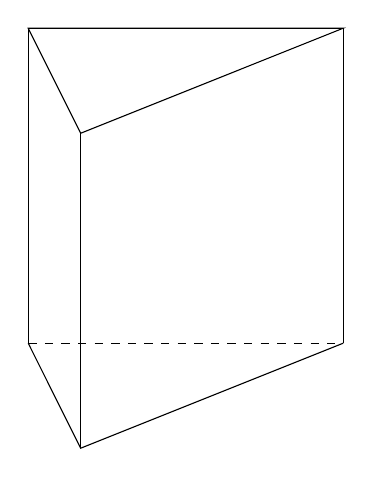
\begin{tikzpicture}
			\coordinate (A) at ($2*(-1, 0, 0)$);
			\coordinate (B) at ($2*(1, 0, 0)$);
			\coordinate (C) at ($2*(0, 0, {sqrt(3)})$);
			\coordinate (H) at ($2*(0, 2, 0)$); %height of shape
			
			\draw (B) -- (C) -- (A);
			\draw [dashed] (A) -- (B);
			
			\draw ($ (A) + (H)$) -- ($ (B) + (H)$) -- ($ (C) + (H)$) -- cycle;
			
			\draw (A)  --+ (H); % (A) -- ($ (A) + (H)$)
			\draw (B) --+ (H);
			\draw (C) --+ (H);
		\end{tikzpicture}
	\end{center}
\end{document}